\documentclass[a4paper, 11pt]{article}\usepackage[]{graphicx}\usepackage[]{color}
%% maxwidth is the original width if it is less than linewidth
%% otherwise use linewidth (to make sure the graphics do not exceed the margin)
\makeatletter
\def\maxwidth{ %
  \ifdim\Gin@nat@width>\linewidth
    \linewidth
  \else
    \Gin@nat@width
  \fi
}
\makeatother

\definecolor{fgcolor}{rgb}{0.345, 0.345, 0.345}
\newcommand{\hlnum}[1]{\textcolor[rgb]{0.686,0.059,0.569}{#1}}%
\newcommand{\hlstr}[1]{\textcolor[rgb]{0.192,0.494,0.8}{#1}}%
\newcommand{\hlcom}[1]{\textcolor[rgb]{0.678,0.584,0.686}{\textit{#1}}}%
\newcommand{\hlopt}[1]{\textcolor[rgb]{0,0,0}{#1}}%
\newcommand{\hlstd}[1]{\textcolor[rgb]{0.345,0.345,0.345}{#1}}%
\newcommand{\hlkwa}[1]{\textcolor[rgb]{0.161,0.373,0.58}{\textbf{#1}}}%
\newcommand{\hlkwb}[1]{\textcolor[rgb]{0.69,0.353,0.396}{#1}}%
\newcommand{\hlkwc}[1]{\textcolor[rgb]{0.333,0.667,0.333}{#1}}%
\newcommand{\hlkwd}[1]{\textcolor[rgb]{0.737,0.353,0.396}{\textbf{#1}}}%

\usepackage{framed}
\makeatletter
\newenvironment{kframe}{%
 \def\at@end@of@kframe{}%
 \ifinner\ifhmode%
  \def\at@end@of@kframe{\end{minipage}}%
  \begin{minipage}{\columnwidth}%
 \fi\fi%
 \def\FrameCommand##1{\hskip\@totalleftmargin \hskip-\fboxsep
 \colorbox{shadecolor}{##1}\hskip-\fboxsep
     % There is no \\@totalrightmargin, so:
     \hskip-\linewidth \hskip-\@totalleftmargin \hskip\columnwidth}%
 \MakeFramed {\advance\hsize-\width
   \@totalleftmargin\z@ \linewidth\hsize
   \@setminipage}}%
 {\par\unskip\endMakeFramed%
 \at@end@of@kframe}
\makeatother

\definecolor{shadecolor}{rgb}{.97, .97, .97}
\definecolor{messagecolor}{rgb}{0, 0, 0}
\definecolor{warningcolor}{rgb}{1, 0, 1}
\definecolor{errorcolor}{rgb}{1, 0, 0}
\newenvironment{knitrout}{}{} % an empty environment to be redefined in TeX

\usepackage{alltt}
\usepackage[OT1]{fontenc}
\usepackage{url}

\usepackage{graphicx}
\usepackage{tikz}
\usetikzlibrary{decorations,arrows,shapes}
\usepackage[margin=0.9in]{geometry}
\usepackage{url}
\usepackage{hyperref}
\usepackage{listings}
\usepackage{xspace}
\usepackage[numbers]{natbib}
%\usepackage[left=3cm,right=3cm,top=2cm,bottom=2cm]{geometry}
\usepackage{amsmath,amsthm,amsfonts,amssymb}
\bibliographystyle{plainnat}
\setlength{\parindent}{0mm}
\setlength{\parskip}{1mm}
\newcommand{\commentout}[1]{}

\renewcommand{\epsilon}{\varepsilon}
\pagestyle{empty}

\pagecolor[rgb]{1.0000000,0.9607843,0.8549020}
\IfFileExists{upquote.sty}{\usepackage{upquote}}{}

\begin{document}

% \VignetteEngine{knitr::knitr}
% \VignetteIndexEntry{gMCP Quick Start Guide}

\title{gMCP Quick Start - an R package for a graphical approach to weighted multiple test procedures} 

\author{Kornelius Rohmeyer}

%\maketitle


% Bibliotheken



\section*{gMCP Quick Start Guide}

\begin{minipage}{0.10\textwidth}

\includegraphics[width=0.9\textwidth]{pictures/rjavaicon64.png}
\end{minipage}
\begin{minipage}{0.90\textwidth}

This package provides functions and graphical user interfaces for graph based
multiple test procedures.
You can use this package completely from the R command line and also completely
from the graphical user interface (GUI) without the need to know any R at all.
This guick start guide only describes the steps to start the GUI.

\end{minipage}

\subsection*{Install and Start}

If you don't already have R on your system, you can download a bundled
version of R and gMCP from \url{http://www.algorithm-forge.com/gMCP/bundle/}.

\begin{minipage}{0.60\textwidth}

Otherwise open \href{http://cran.r-project.org/bin/windows/base/release.htm}{R}
and type \texttt{install.packages("gMCP")} into the R Console, select an arbitrary mirror and gMCP will be downloaded and installed.

From now on you can start the gMCP graphical user interface by entering the following commands into the R Console:

%\scriptsize
\begin{knitrout}
\definecolor{shadecolor}{rgb}{0.969, 0.969, 0.969}\color{fgcolor}\begin{kframe}
\begin{alltt}
\hlkwd{library}\hlstd{(gMCP)}
\hlkwd{graphGUI}\hlstd{()}
\end{alltt}
\end{kframe}
\end{knitrout}

%\normalsize

\end{minipage}
\begin{minipage}{0.40\textwidth}
\begin{flushright}
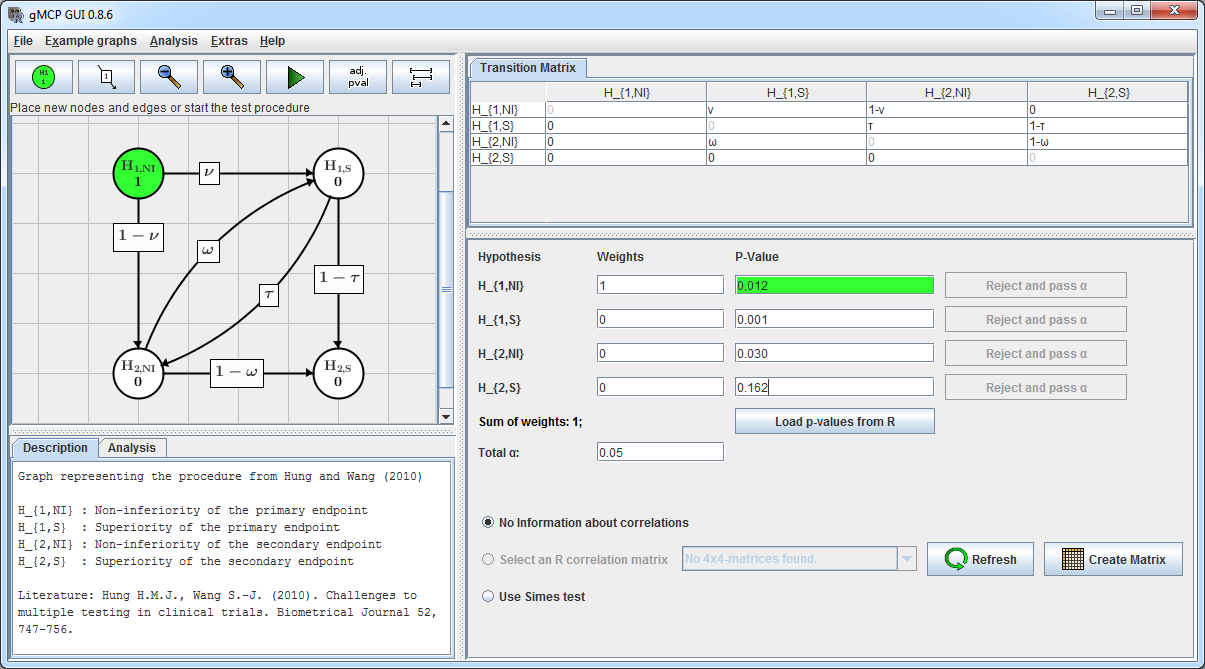
\includegraphics[width=0.9\textwidth]{pictures/FullFeaturedGUI.png}
\end{flushright}
\end{minipage}

\subsection*{Creation of the graph}

Use the first two buttons of the icon panel to create a graph or 
select one of the common test procedures from our example menu, that include the 
fixed sequence test, fallback procedure, improved fallback procedure, 
parallel gatekeeping, improved parallel gatekeeping, truncated Holm procedure and many more.

\subsection*{Test procedure, CI and adjusted p-values}

After you have created or loaded your graph you can start the test procedure and 
calculate confidence intervals or adjusted p-values by using the last three buttons of the icon panel.

For all further questions take a look at the help menu, the \href{http://cran.r-project.org/web/packages/gMCP/gMCP.pdf}{manual} or mail us at: 

\begin{center}\href{mailto:help@small-projects.de}{\texttt{help@small-projects.de}}\end{center}

\end{document}
